%%%%%%%%%%%%%%%%%%%%%%%%%%%%%%%%%%%%%%%%%%%%%%%%%%%%%%%%%%%%%%%%%%%%%%%%%%%%%%%%%%%%%%%%%%%%%%%%
% Integral 
%%%%%%%%%%%%%%%%%%%%%%%%%%%%%%%%%%%%%%%%%%%%%%%%%%%%%%%%%%%%%%%%%%%%%%%%%%%%%%%%%%%%%%%%%%%%%%%%
\section{Integralrechnung\formelbuchviolet{492}}

\subsection{Bestimmtes Integral\formelbuchviolet{505}}
  $I = \int\limits_{a}^{b}{f(\widetilde{x})}d\widetilde{x} = \lim\limits_{d(Z) \rightarrow 0}S(Z) = \lim\limits_{d(Z) \rightarrow 0}O(Z)  = \lim\limits_{d(Z) \rightarrow 0}U(Z)  $ \\ 
	$x$: Integrationsver"anderliche, $f$: Integranden, $[a,b]$: Integrationsintervall, $a/b$: untere bzw. obere Integrationsgrenze

\subsection{Integrierbarkeit}
	\begin{minipage}[c]{10cm}
		\begin{center}
			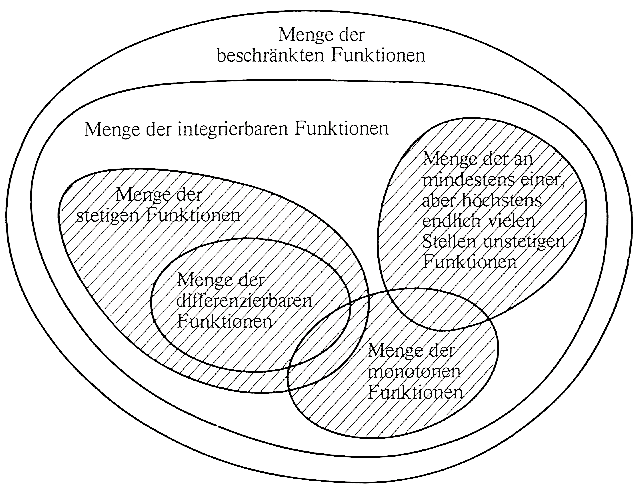
\includegraphics[width=6cm]{./bilder/integral_mengen.png} 
		\end{center}
	\end{minipage}
	\begin{minipage}[c]{7cm}
		\textbf{Schranken vom Integral:}\\
		$g_1(x) \leq f(x) \leq g_2(x)$\\
		$\int\limits_{a}^{b} g_1(\widetilde{x}) d\widetilde{x} \leq \int\limits_{a}^{b} f(\widetilde{x}) d\widetilde{x} \leq \int\limits_{a}^{b} g_2(\widetilde{x}) d\widetilde{x}$
	\end{minipage}
	
\subsection{Integralregeln\formelbuchviolet{494}}
	$\int\limits_a^b \widetilde{x}^n d\widetilde{x}=\frac{1}{n+1}(b^{n+1}-a^{n+1})$
	
\subsection{Fl"acheninhalt\formelbuchviolet{507}}
	Inhalt der Fl"ache unter dem Graphen $f: A = \int\limits_a^b |f(\widetilde{x})| d\widetilde{x}$ \\
	$A = A_1 - A_2 = \int\limits_a^b f_1(\widetilde{x}) d\widetilde{x} - \int\limits_a^b f_2{\widetilde{x}} d\widetilde{x} \qquad \text{gilt auch wenn die Funktionen }f_1 \text{ oder }f_2 \text{ negativ werden.}$

\subsection{Mittelwertsatz\formelbuchviolet{509}}
	$f$ auf $[a,b] \mbox{ stetig} \Rightarrow \mbox{ mind. eine Stelle } \xi \in (a,b)\mbox{ mit } \int\limits_a^b{f(\widetilde{x})}d\widetilde{x}=(b-a)f(\xi) 
	\Rightarrow h = \frac{1}{b-a} \int\limits_a^b{f(\widetilde{x})}d\widetilde{x}$ \\
	$h \hat{=}$ Mittelwert der Funktion

\subsection{Integralfunktion}
	$c \in [a,b]$ und $f(x)$ "uber $[a,b]$ integrierbar: $I: x \mapsto I(x) = \int\limits_c^x{f(\widetilde{t})}d\widetilde{t}$
	
\subsubsection{Differenzierbarkeit\formelbuchviolet{508}} 
	\begin{minipage}[t]{9.5cm}		
			$ \frac{d}{dx} \int\limits_{a(x)}^{b(x)} f(\widetilde{t}) d\widetilde{t} = f(b(x)) \cdot b'(x) - f(a(x)) \cdot a'(x) $
	\end{minipage}
	\begin{minipage}[t]{5cm} 	
			$ \qquad \frac{d}{dx} \int\limits_c^x f(\widetilde{t})d\widetilde{t} = f(x)$
	\end{minipage}
	
\subsection{Unbestimmtes Integral\formelbuchviolet{492}}
	$F(x) + C = \int{f(\widetilde{x})}d\widetilde{x}$

\subsection{Stammfunktion\formelbuchviolet{492}}
	Jede auf $[a,b]$ differenzierbare Funktion $F$ nennt man Stammfunktion, wenn $F'=f$.\\
	$I(x) \subset F(x)$

\subsection{Rechenregeln\formelbuchviolet{495}}
	\begin{tabular}{l c}
		$\int\limits_a^b f(\widetilde{x}) d\widetilde{x} = F(b) - F(a)$ & $|\int\limits_a^b f(x) dx| \leq \int\limits_a^b |f(\widetilde{x})| d\widetilde{x}$\\
		$\int\limits_a^b f(\widetilde{x}) d\widetilde{x} = \int\limits_0^b f(\widetilde{x}) d\widetilde{x} - \int\limits_0^a f(\widetilde{x})d\widetilde{x} = \int\limits_0^b f(\widetilde{x}) d\widetilde{x} - (-1) \cdot \int\limits_a^0 f(\widetilde{x})d\widetilde{x}$
	\end{tabular}

